% !TEX root = ../main.tex
\chapter{Noise analysis of PSR~J1640+2224} \label{chpt:risultati}

\subsection{Validation of Discovery} \label{sec:validazione}

All the analyses of this thesis are performed with \textsc{Discovery}. Since
it is a recent code, we first verify that it reproduces the results of
\textsc{Enterprise}, the reference software introduced in
Section~\ref{sec:software}. We analyze the DR2low data of PSR~J1640+2224
with both codes, using the reference noise model of Section~\ref{NM}, the
priors of Section~\ref{sec:bayes} and the same sampler, so that the only
difference is the implementation of the likelihood.

The posterior distributions are compared in
Figure~\ref{fig:disc_vs_ent}. The contours obtained with the two codes
overlap in all the panels, and the marginalized posteriors of the six
parameters have the same shape. The medians and the intervals between the
16th and the 84th percentiles, which are the values quoted throughout this
chapter, are also in agreement. For example, the amplitude of the intrinsic
red noise is $\log_{10}A_{\rm RN} = -13.24^{+0.09}_{-0.10}$ with both codes.
The largest difference is found for the spectral index of the DM variations,
$\gamma_{\rm DM} = 4.12^{+2.33}_{-2.28}$ with \textsc{Discovery} and
$\gamma_{\rm DM} = 3.94^{+2.48}_{-2.12}$ with \textsc{Enterprise}, and it is
much smaller than the width of the posterior. The effective number of
samples of Eq.~\eqref{eq:neff} is $1141$ for the \textsc{Discovery} chain and
$1557$ for the \textsc{Enterprise} one, so differences of this size are
expected from the finite length of the chains.

The agreement also holds for the non-Gaussian features of the posterior,
namely the two peaks of the DM parameters and the L-shaped contours between
the DM and the scattering parameters, which are discussed below. We conclude
that \textsc{Discovery} reproduces the results of \textsc{Enterprise} for
this model, and we use it for all the following analyses.

\begin{figure}[H]
    \centering
    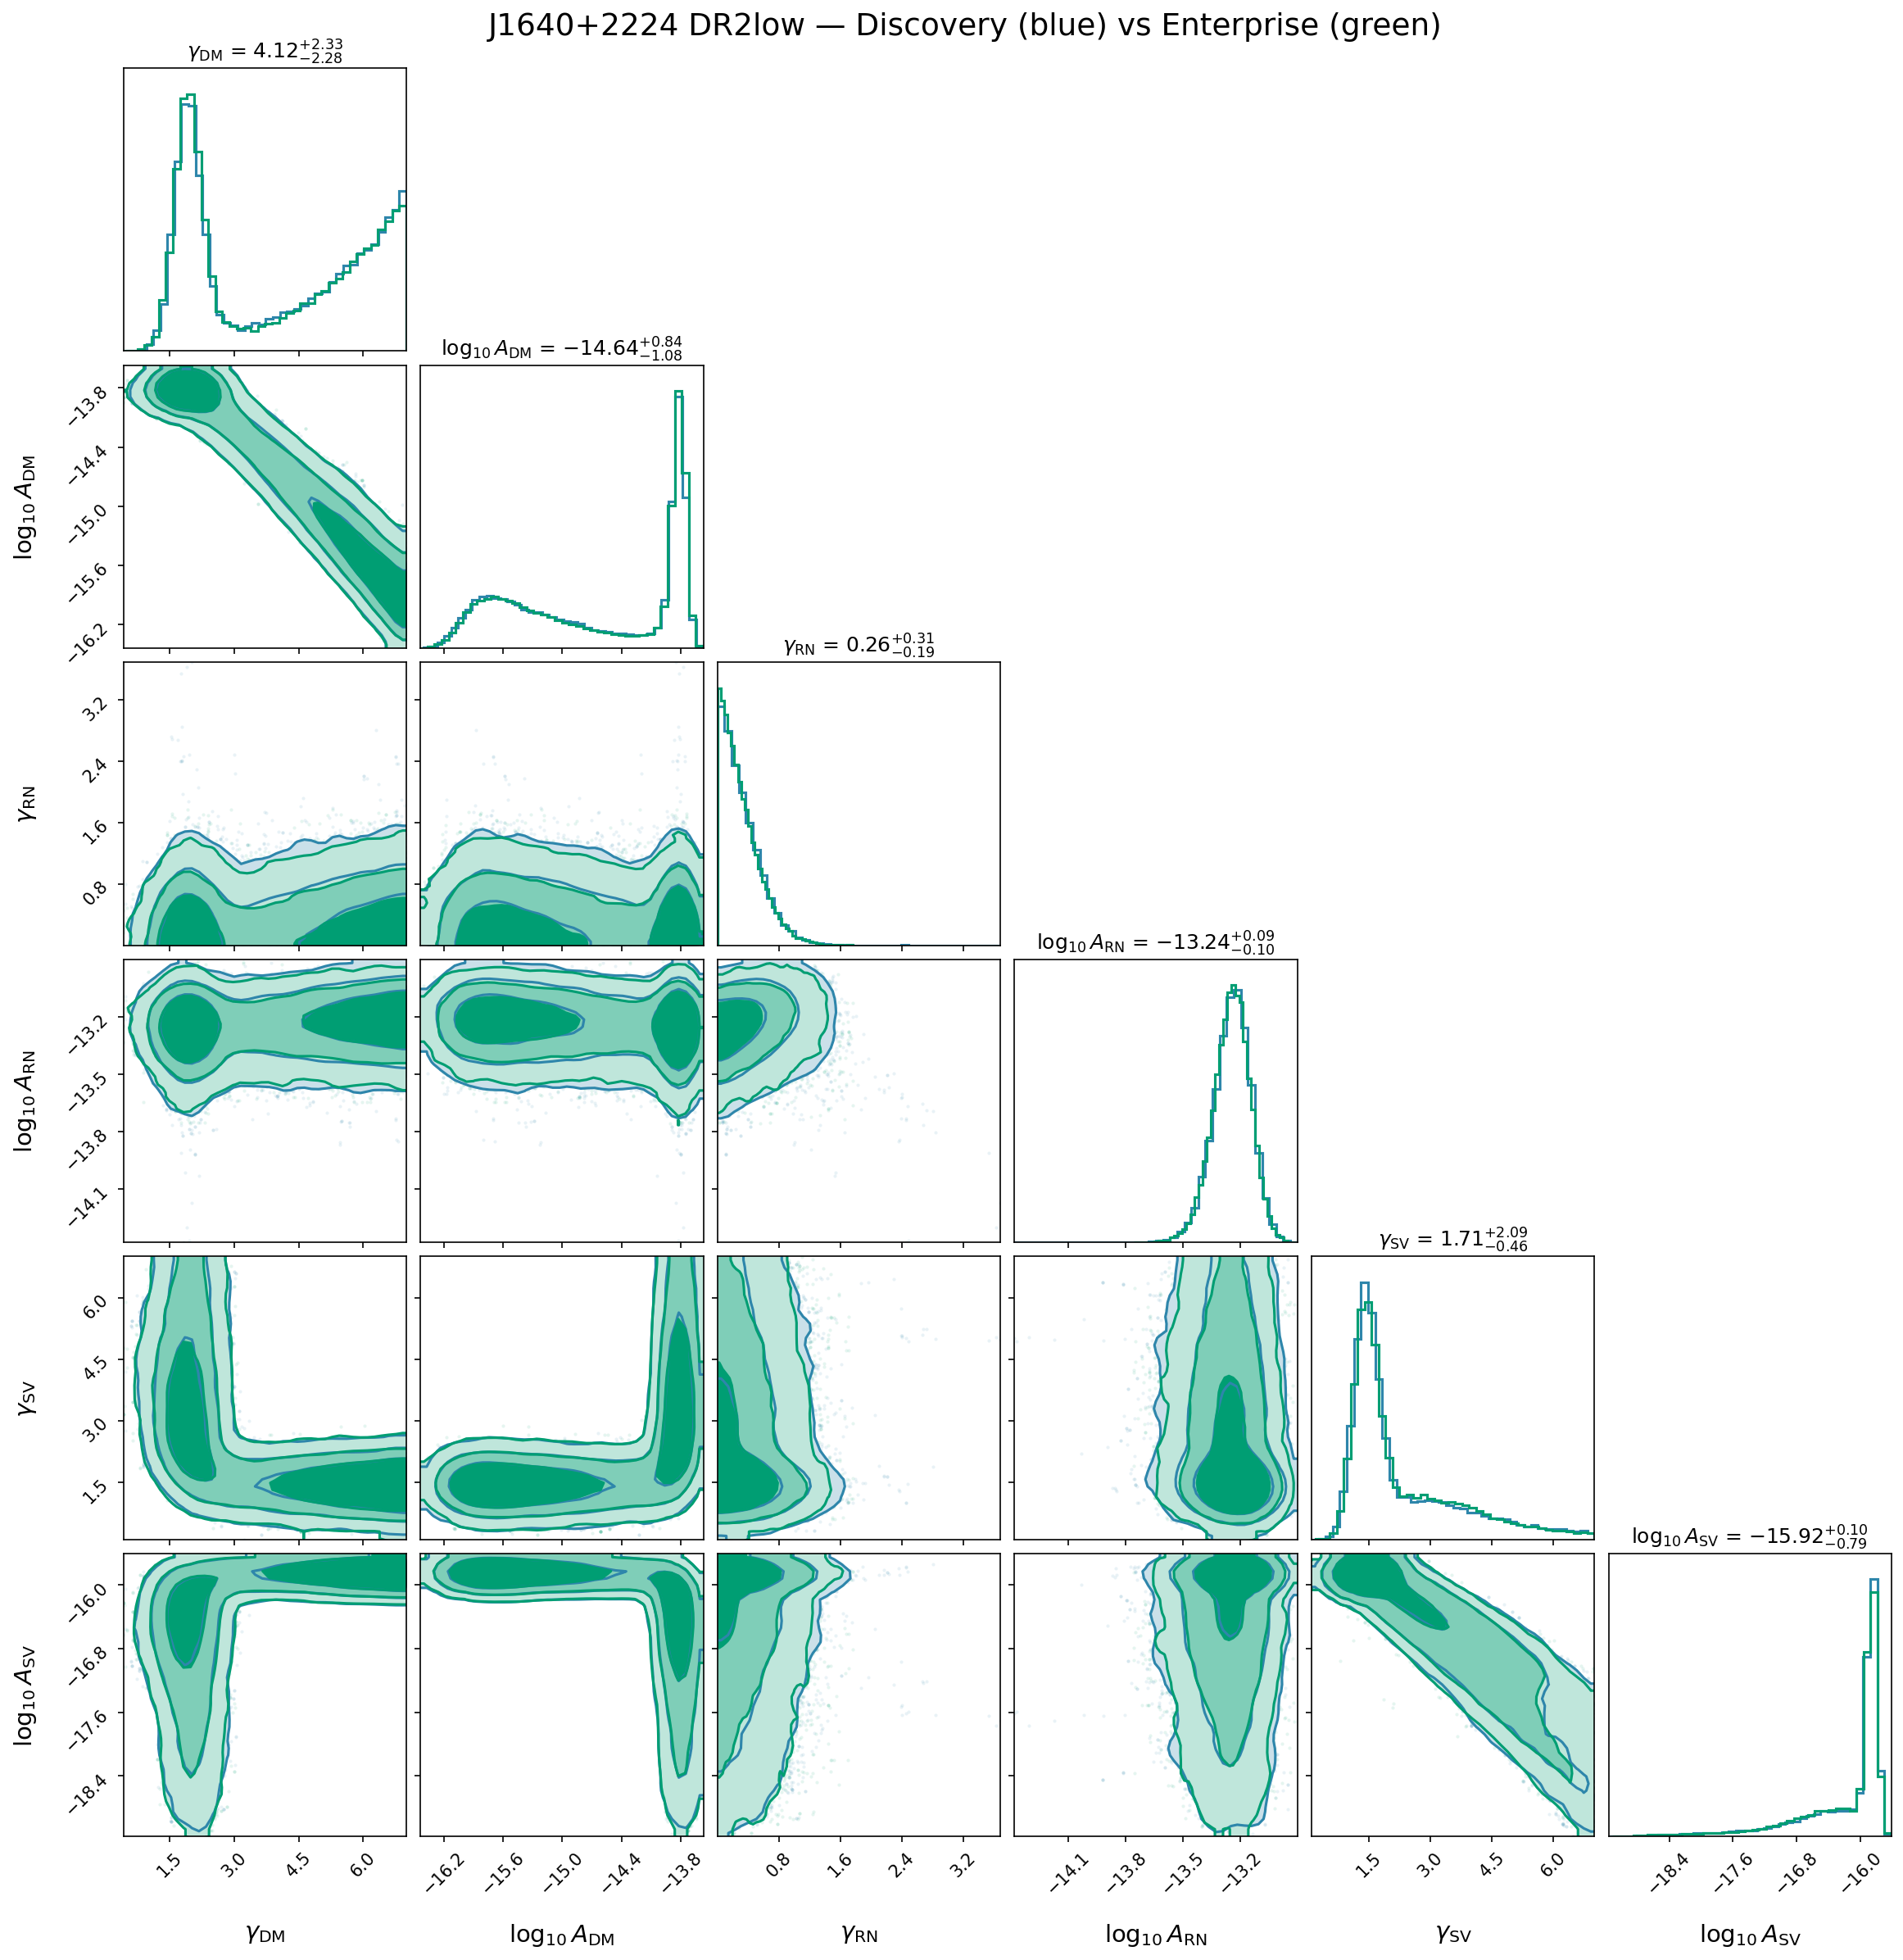
\includegraphics[width=\textwidth]{Figure/cap5/01_discovery_vs_enterprise.png}
    \caption{Posterior distributions of the six noise parameters of
    PSR~J1640+2224 obtained from the DR2low data with \textsc{Discovery}
    (blue) and with \textsc{Enterprise} (green). The contours enclose $68\%$,
    $95\%$ and $99.7\%$ of the probability. The values above the diagonal
    panels are the median and the 16th and 84th percentiles of the
    \textsc{Discovery} chain.}
    \label{fig:disc_vs_ent}
\end{figure}
